\documentclass{article}
\usepackage{graphicx}
\usepackage{amsmath}

\begin{document}

\title{Backbone Determination in a Wireless Sensor Network}
\author{Jake Carlson}
\date{February 18, 2018}
\maketitle

\abstract
A report on implementing algorithms to partition a random geometric graph into bipartite subgraphs. Three different graph geometries are explored: unit square, unit disk, and unit sphere. Nodes are uniformly distributed in the geometry. Then the edges are determined and ...
\newpage

\tableofcontents
\newpage

\section{Executive Summary}

    \subsection{Introduction}
    Random geometric graphs (RGGs) are useful for simulating wireless sensor networks placed in different topologies. This project examines three different geometries: Square, Disk, and Sphere. The user supplies parameters for how many nodes they want in the network and how many connections they want for each node. Then, the simulation finds the average radius needed for that number of connections, finds multiple backbones for the RGG, and displays the results graphically.

    \subsection{Environment Description}
    The data structures and topologies for this simulation are implemented in Python2.7. The graphics are done using Processing.py. All development and benchmarking has been done on a 2014 MackBook Pro with a 3 GHz Intel Core i7 processor and 16 GB of DDR3 RAM.

\section{Reduction to Practice}

    \subsection{Data Structure Design}
    The primary data structure used for this project is an adjacency list. However, to allow for constant time lookup of edges of a node, I used a Python dictionary where the keys are nodes and the values are a list of adjacent nodes.
    \par
    In order to make this project maintainable as it is built on along the semester, I used the object-oriented capabilities Python has to offer to design the different geometries. I start with a base Topology class that creates the interface Processing uses to draw the graphs. This base class implements all of the methods needed for node placement and edge detection in 2D graphs. Then, I create three subclasses: Square, Disk, and Sphere.
    \par
    The Square and Disk topologies simply need to override the methods for generating nodes and calculating the node radius needed for the desired average degree. The Sphere subclass needs to override a few additional functions because it exists in a 3D space. Other than the methods for generating nodes and calculating the node radius, it also needs to override the function used to draw the graph so that Processing will render the graph properly in 3D.

    \subsection{Algorithm Descriptions}

        \subsubsection{Node Placement}
        A different node placement algorithm is required for each of the geometries. For the Square, the coordinates for each node are generated as two random numbers taken from a unifrom distribution on the range $[0,1]$. All of these points are guaranteed to be in the unit square.
        \par
        For the Disk, a similar method is used. The coordinates for nodes are randomly sampled from a uniform distribution; however, if a node has a distance from the center of the Disk greater than the radius of 1, the coordinates for that node are resampled.
        \par
        For the Sphere a different method must be used so that all of the nodes are placed on the surface of the Sphere and the volume is vacant. For this geometry, I used the following equations:
        \begin{align}
            x &= \sqrt{1-u^2}\cos\theta \\
            y &= \sqrt{1-u^2}\sin\theta \\
            z &= u
        \end{align}
        where $\theta \in [0,2\pi]$ and $u \in [-1,1]$. This is guaranteed to uniformly distribute nodes on the surface area of the sphere \cite{spherepoints}.
        \par
        All of these algorithms can be solved in $\Theta\left(n\right)$ where $n = |V|$ because each node only needs to be assigned a position once.

        \subsubsection{Edge Determination}
        There are several methods for finding the edges in the graph. The brute force method checks every node, and for each node checks all other nodes to see if they are close enough to form an edge. The brute force method is $\Theta\left(n^2\right)$ where $n = |V|$.
        \par
        The second method to find the edges is the sweep method. This method first sorts the nodes along the x-axis. Then, for any node, we only need to search left and right until the distance along the x-axis is greater than the connection radius for the nodes. This dramatically reduces the search space. The sweep method is $O\left(n lg(n) + 2rn^2\right)$ where $n = |V|$ and $r$ is the connection radius. The $n lg(n)$ portion is for the sorting and the $2rn^2$ portion is for measuring the distance between nodes in a sweep step.
        \par
        The final method to find edges is the cell method. This method places the nodes into cells of area $r \times r$ based on their position in the topology. When the edge detection runs, each node needs to be visited once, but only the cell the node populates and the neighboring cells need to be searched for connections.

        % TODO: update for 3D algos

    \subsection{Algorithm Engineering}

        \subsubsection{Node Placement}
        It is easy to implement the algorithms for placing nodes in the different geometries using Python's math library. This library offers functions for sampling points on a uniform distribution. For the Square, sampling on a range $[0,1]$ is sufficient for all of the nodes. Since each node only needs to be placed once, this runs at $\Theta(n)$ where $n = |V|$.
        \par
        For the Disk, the node needs to be resampled if it is too far from the center. To do this, the distance funciton is used to find the distance between the node and the center. If the node is further than $1$ from the center, node generation falls into a while loop which iterates until the node is within the unit circle. Since nodes are taken from a uniform distribution, the number of nodes that will need to be resampled is approximately equal to the ratio of the area of the square that circumscribes the unit circle which falls outside of the unit circle to the total area of the square. This is given by:
        \begin{align}
            \frac{(2r)^2-\pi r^2}{(2r)^2} = \frac{4-\pi}{4} = 0.2146
        \end{align}
        Since the placement algorithm for each node of the Disk will iterate until the node falls within the unit circle, the total number of iterations $I$ can be found as the sum of the geometric series:
        \begin{align}
            I = \sum_{k=0}^{\infty} n (0.2146)^k = \frac{n}{1-0.2146} = 1.273n
        \end{align}
        where $n = |V|$. This shows this implementation is $\Theta\left(n\right)$.
        \par
        For the node placement algorithm of the Sphere, again the math library in Python makes this easy. Each node needs two random values pulled from a uniform distribution, two square root operations, one sine operation, and one cosine operation. Each node only needs to be placed once so the runtime of this algorithm is $\Theta(n)$ where $n = |V|$.

        \subsubsection{Edge Determination}

    \subsection{Verification}

    % \subsection{RGG Generation}
    %
    %     \subsubsection{Edge Determination}
    %
    % \subsection{Graph Coloring}
    %
    % \subsection{Backbone Selection}

\section{Results Summary}

\newpage

\begin{thebibliography}{10}
    \bibitem{spherepoints}
    Weisstein, Eric W., Wolfram MathWorld
    \textit{Sphere Point Picking}
    \texttt{http://mathworld.wolfram.com/SpherePointPicking.html}

\end{thebibliography}

\newpage

\section{Appendix}

\begin{center}
    \begin{figure}
        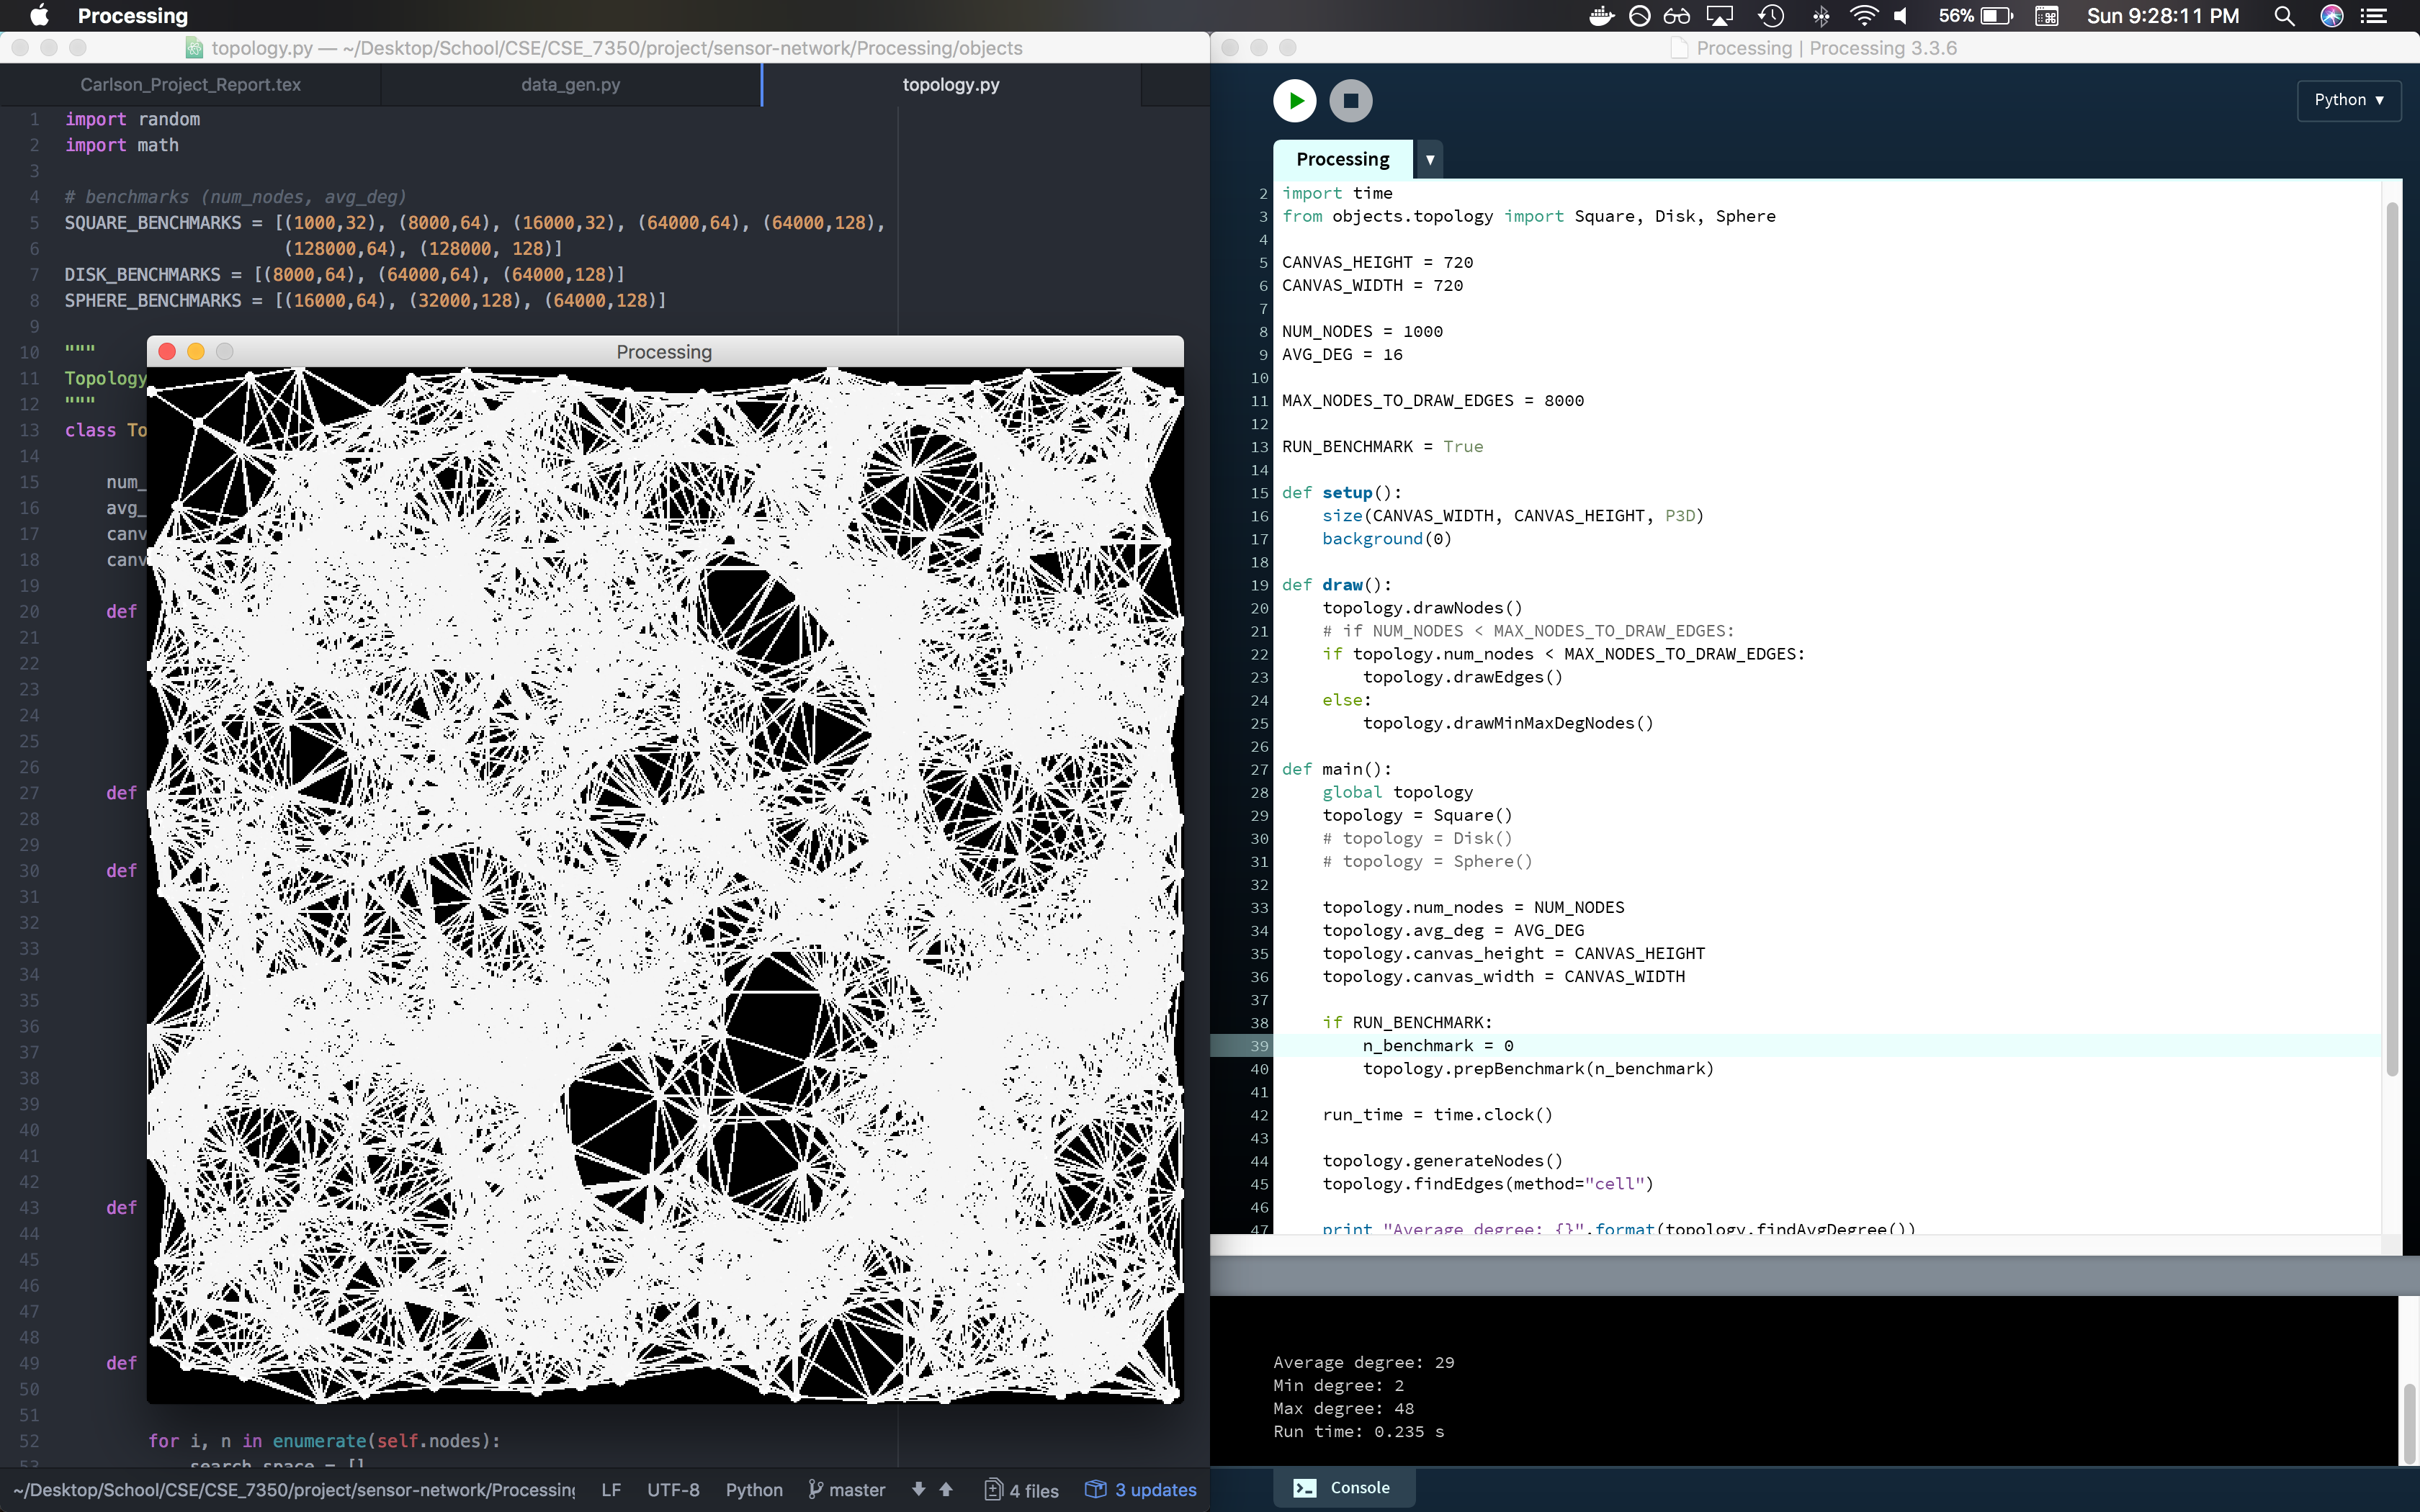
\includegraphics[scale=0.45]{./images/square_0.png}
        \caption{Square Benchmark Number 0. 1000 Nodes, Average Degree of 32}
        \label{square0}
    \end{figure}
\end{center}

\begin{center}
    \begin{figure}
        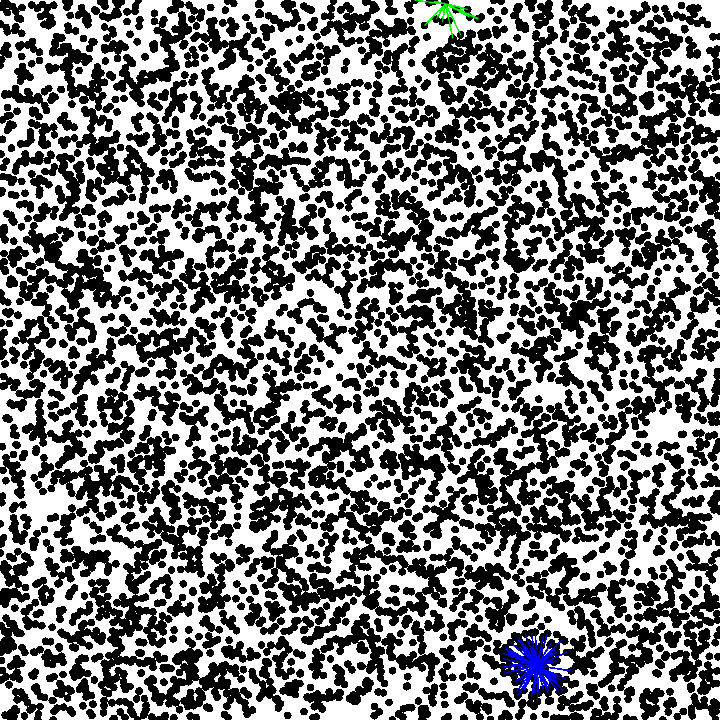
\includegraphics[scale=0.45]{./images/square_1.png}
        \caption{Square Benchmark Number 1. 8000 Nodes, Average Degree of 64}
        \label{square1}
    \end{figure}
\end{center}

\begin{center}
    \begin{figure}
        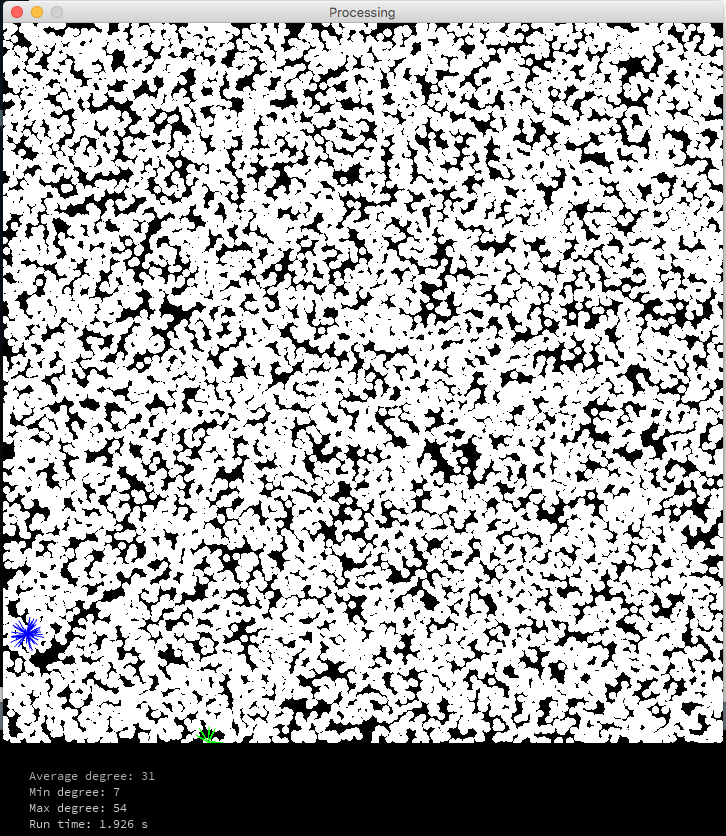
\includegraphics[scale=0.45]{./images/square_2.png}
        \caption{Square Benchmark Number 2. 16000 Nodes, Average Degree of 32}
        \label{square2}
    \end{figure}
\end{center}

\begin{center}
    \begin{figure}
        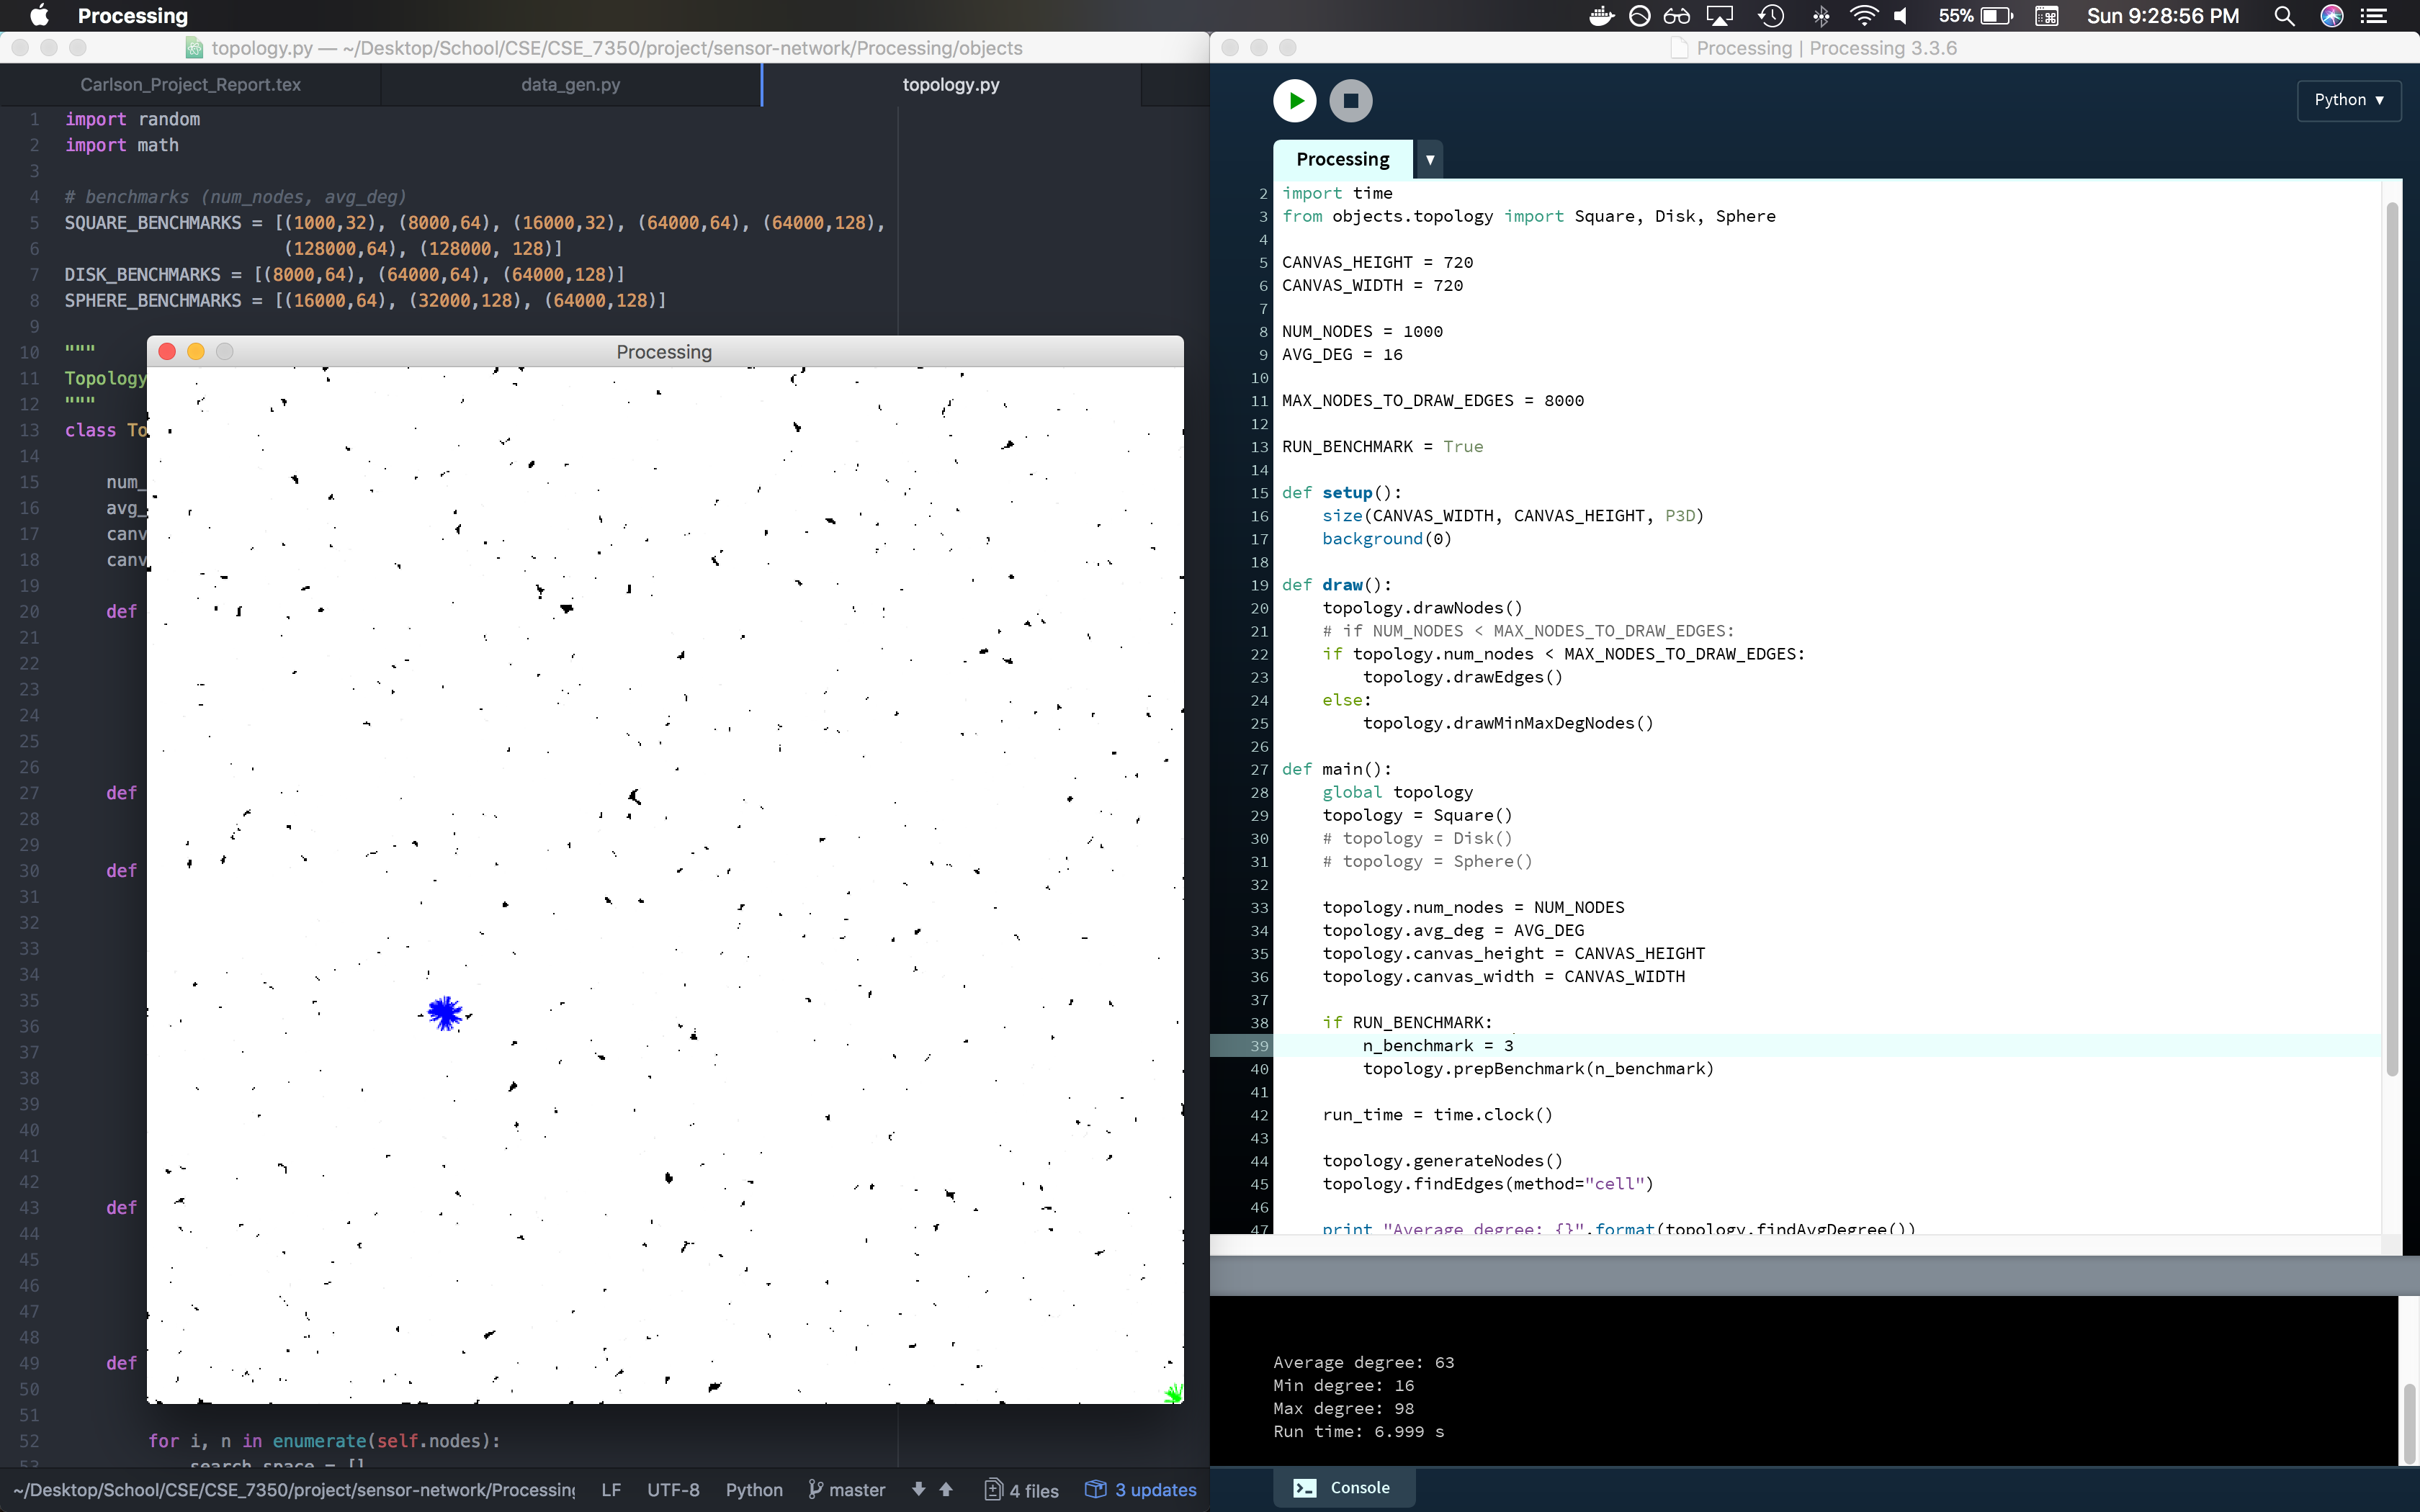
\includegraphics[scale=0.45]{./images/square_3.png}
        \caption{Square Benchmark Number 3. 64000 Nodes, Average Degree of 64}
        \label{square3}
    \end{figure}
\end{center}

\begin{center}
    \begin{figure}
        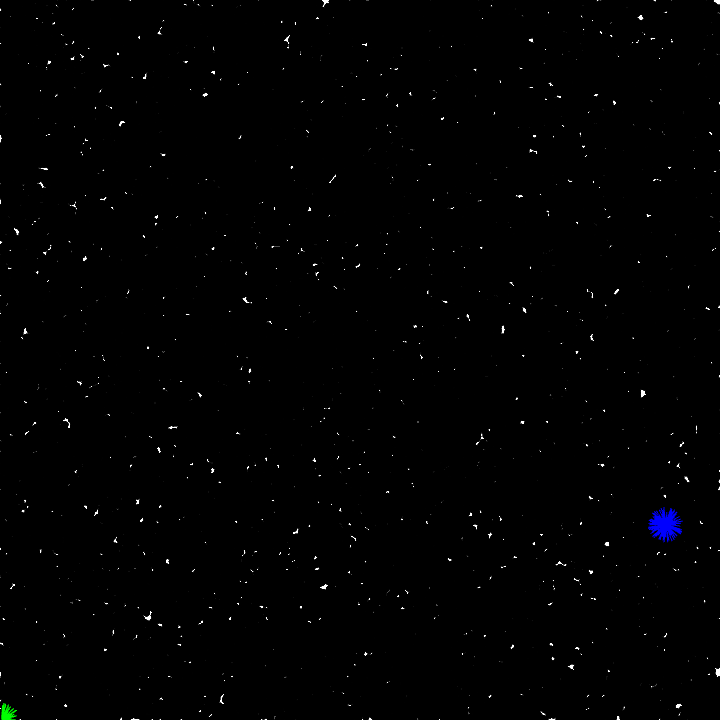
\includegraphics[scale=0.45]{./images/square_4.png}
        \caption{Square Benchmark Number 4. 64000 Nodes, Average Degree of 128}
        \label{square4}
    \end{figure}
\end{center}

\begin{center}
    \begin{figure}
        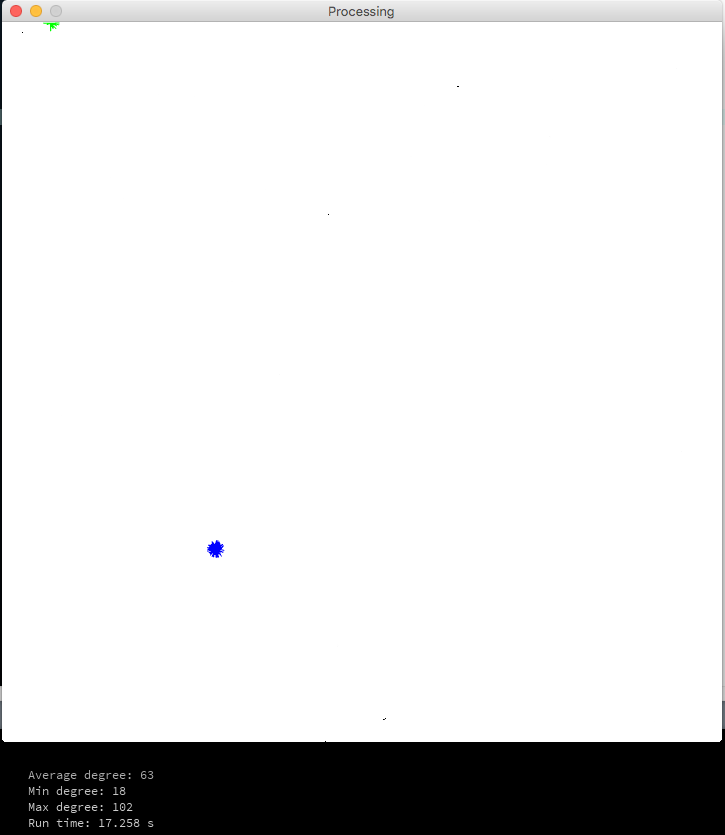
\includegraphics[scale=0.45]{./images/square_5.png}
        \caption{Square Benchmark Number 5. 128000 Nodes, Average Degree of 64}
        \label{square5}
    \end{figure}
\end{center}

\begin{center}
    \begin{figure}
        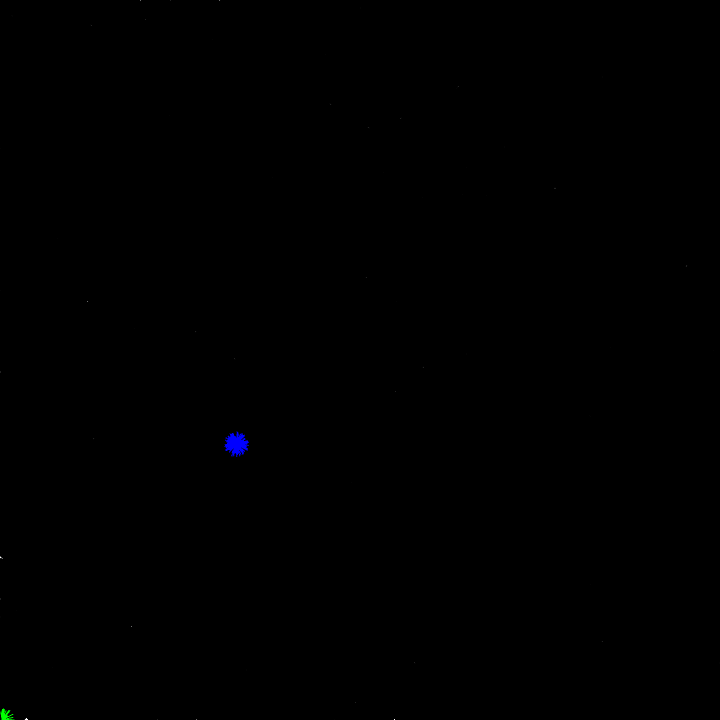
\includegraphics[scale=0.45]{./images/square_6.png}
        \caption{Square Benchmark Number 6. 128000 Nodes, Average Degree of 128}
        \label{square6}
    \end{figure}
\end{center}

\begin{center}
    \begin{figure}
        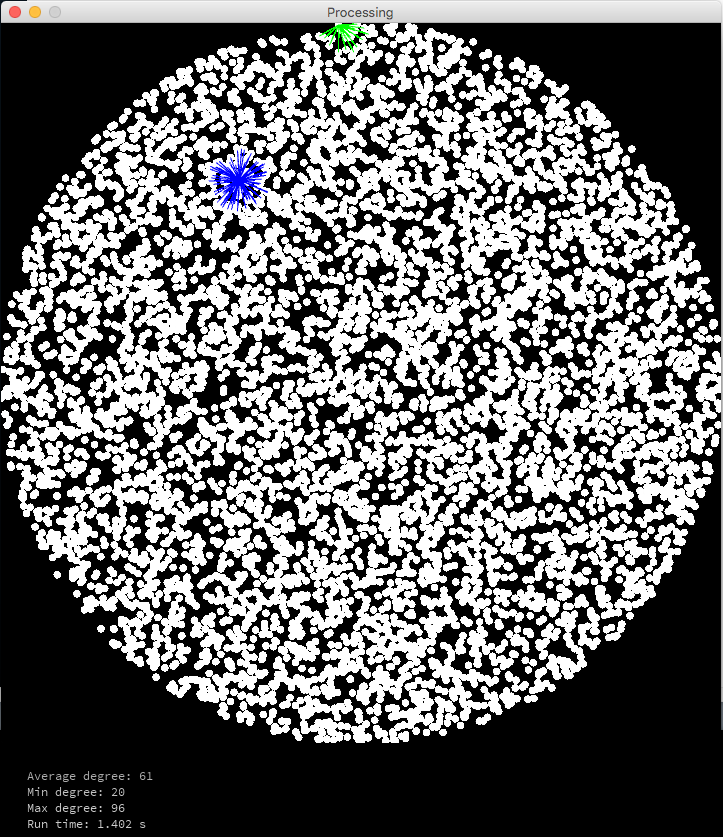
\includegraphics[scale=0.45]{./images/disk_0.png}
        \caption{Disk Benchmark Number 0. 8000 Nodes, Average Degree of 64}
        \label{disk0}
    \end{figure}
\end{center}

\begin{center}
    \begin{figure}
        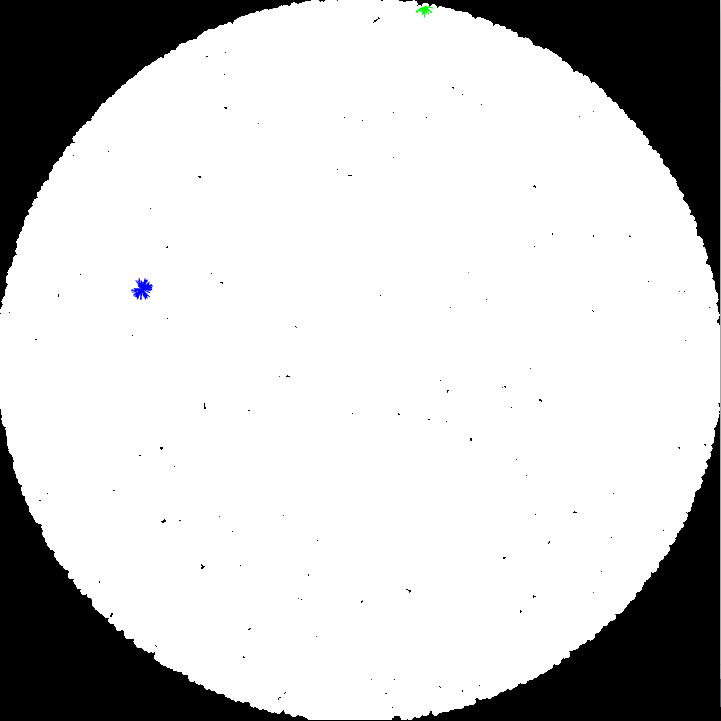
\includegraphics[scale=0.45]{./images/disk_1.png}
        \caption{Disk Benchmark Number 1. 64000 Nodes, Average Degree of 64}
        \label{disk1}
    \end{figure}
\end{center}

\begin{center}
    \begin{figure}
        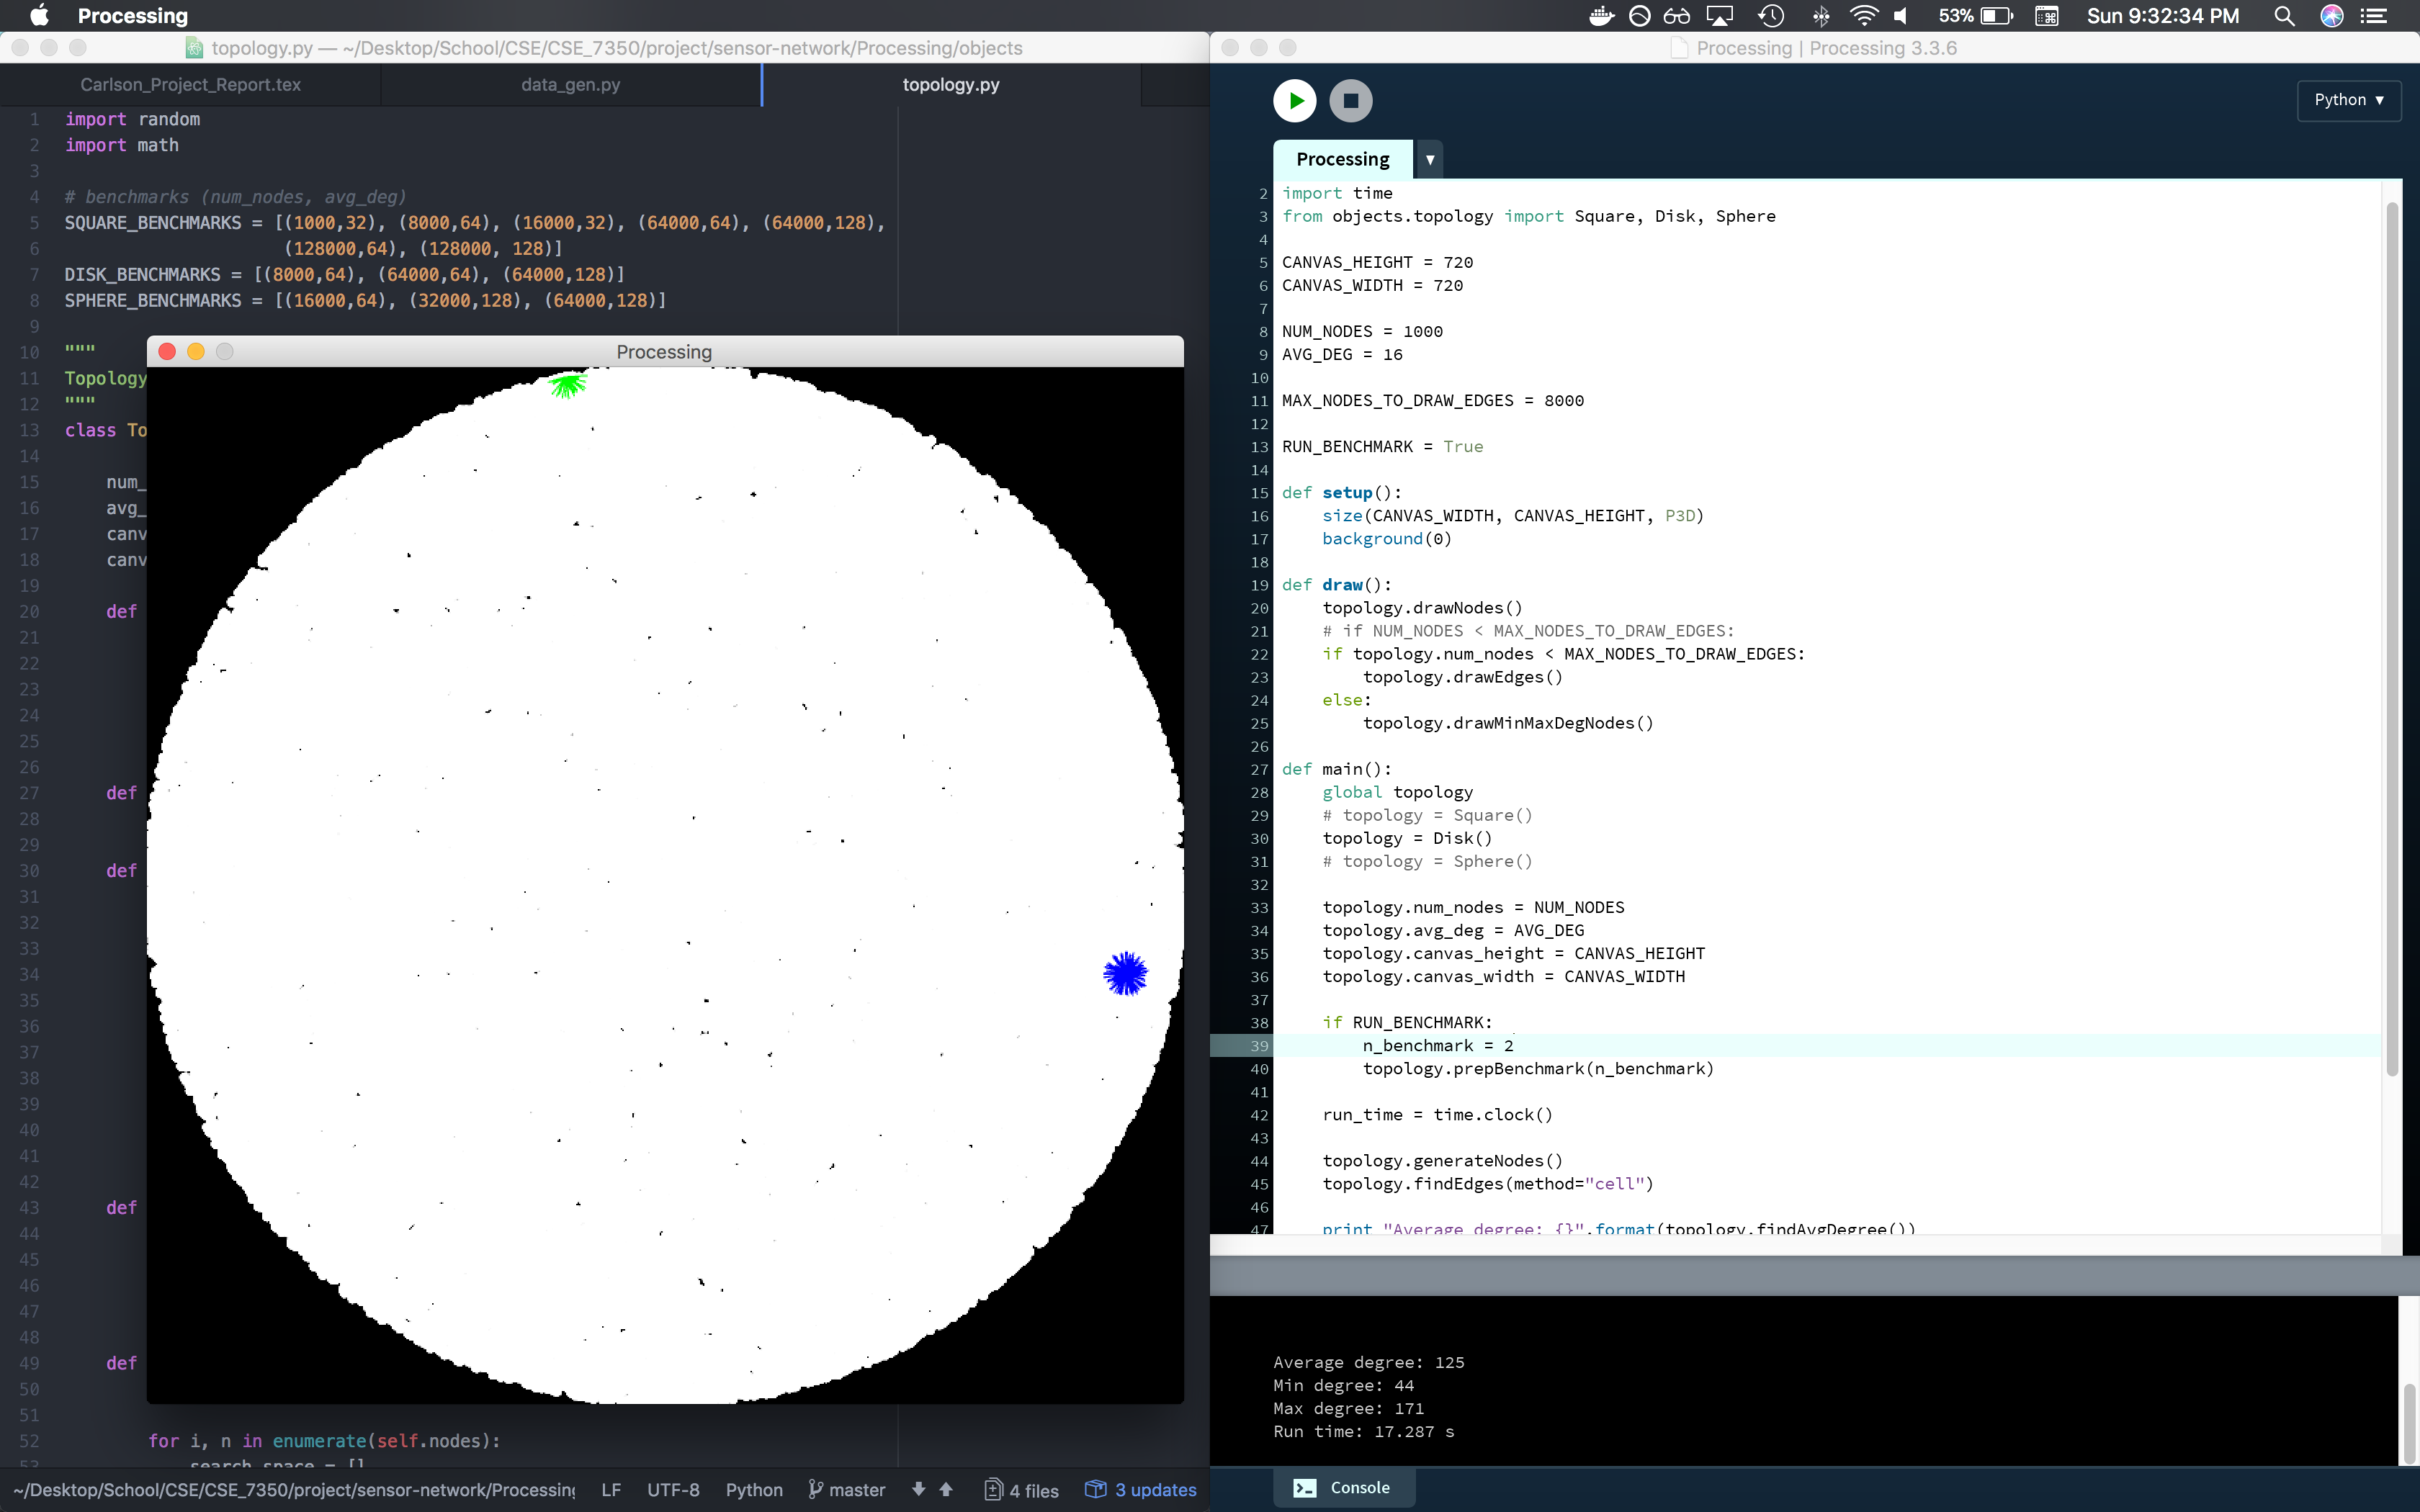
\includegraphics[scale=0.45]{./images/disk_2.png}
        \caption{Disk Benchmark Number 2. 64000 Nodes, Average Degree of 128}
        \label{disk2}
    \end{figure}
\end{center}

\begin{center}
    \begin{figure}
        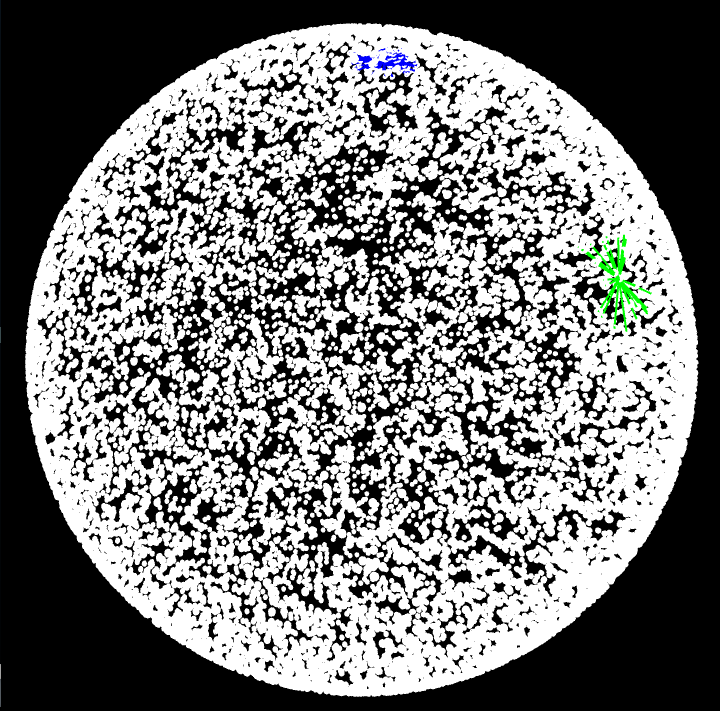
\includegraphics[scale=0.45]{./images/sphere_0.png}
        \caption{Sphere Benchmark Number 0. 16000 Nodes, Average Degree of 64}
        \label{sphere0}
    \end{figure}
\end{center}

\begin{center}
    \begin{figure}
        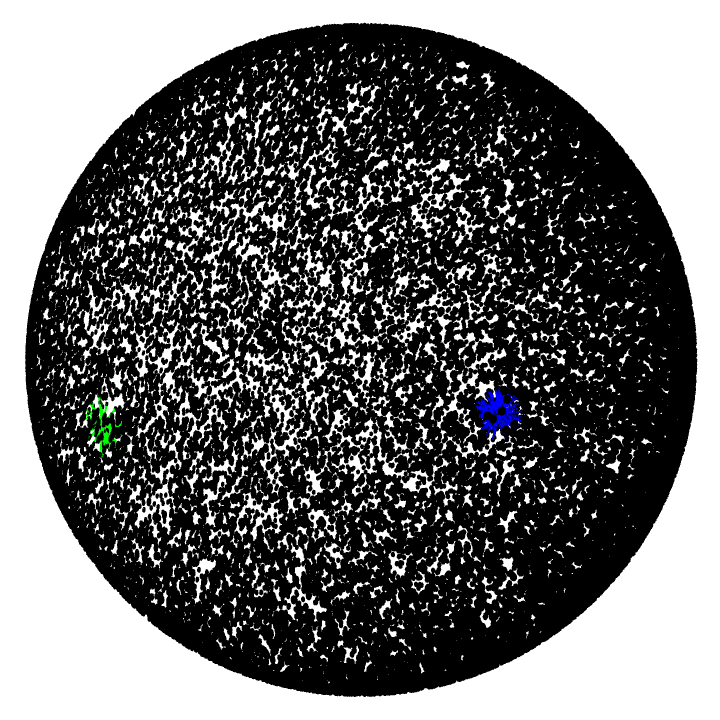
\includegraphics[scale=0.45]{./images/sphere_1.png}
        \caption{Sphere Benchmark Number 1. 32000 Nodes, Average Degree of 128}
        \label{sphere1}
    \end{figure}
\end{center}

\begin{center}
    \begin{figure}
        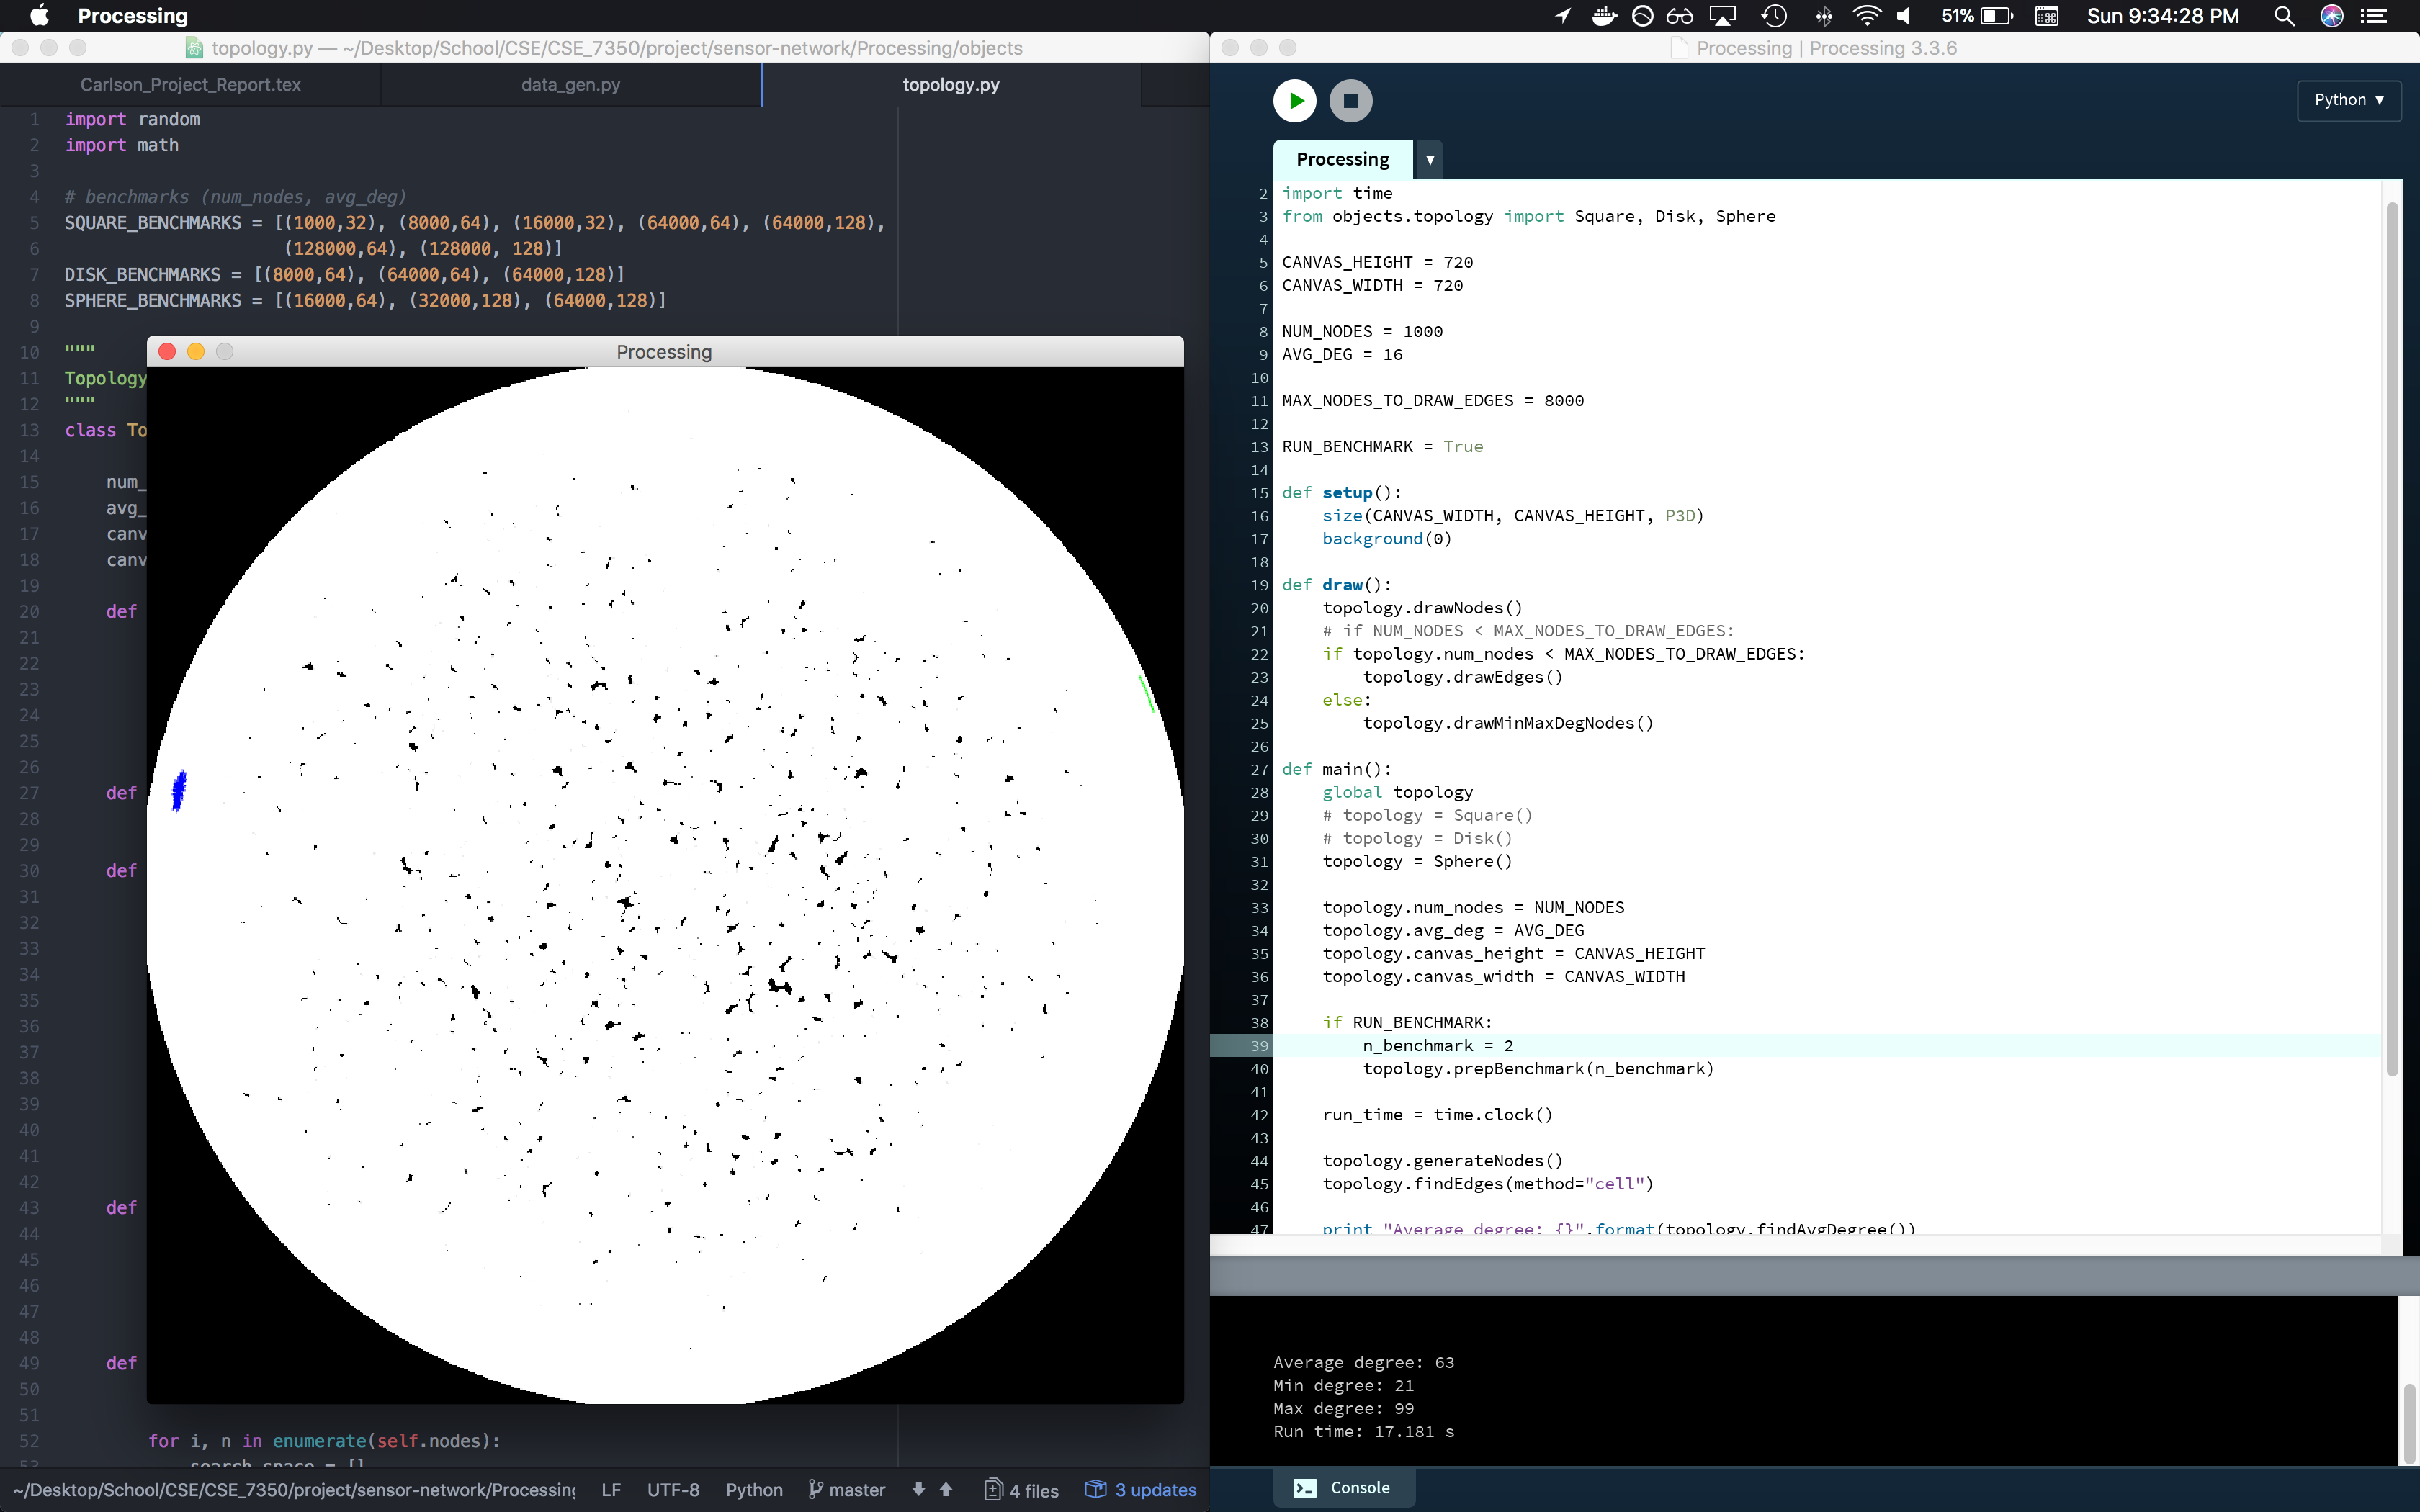
\includegraphics[scale=0.45]{./images/sphere_2.png}
        \caption{Sphere Benchmark Number 2. 64000 Nodes, Average Degree of 128}
        \label{sphere2}
    \end{figure}
\end{center}

\end{document}
